\documentclass[aspectratio=169]{beamer}

\usetheme{default}
\usepackage{booktabs}
\usepackage{graphicx}
\usepackage{amsmath}
\usepackage{xcolor}
\usepackage{tikz}
\usepackage{CJKutf8}
\usepackage[T1]{fontenc}
\usepackage{lmodern}         % Latin Modern serif font
\usefonttheme{serif}
\usepackage{appendixnumberbeamer}
\usepackage{hyperref}
\pdfstringdefDisableCommands{\let\translate\@firstofone}
\newcommand{\sym}[1]{\ensuremath{^{#1}}}
\newcommand{\zh}[1]{~{\tiny\mbox{\begin{CJK}{UTF8}{gbsn}#1\end{CJK}}}}

% B&W palette
\definecolor{mainblack}{HTML}{1A1A1A}
\definecolor{darkgray}{HTML}{404040}
\definecolor{lightgray}{HTML}{EFEFEF}

% No colored backgrounds — white slides, black text
\setbeamercolor{background canvas}{bg=white}
\setbeamercolor{normal text}{fg=mainblack}
\setbeamercolor{frametitle}{bg=white, fg=mainblack}
\setbeamercolor{title}{fg=mainblack}
\setbeamercolor{subtitle}{fg=darkgray}
\setbeamercolor{author}{fg=darkgray}
\setbeamercolor{alerted text}{fg=mainblack}
\setbeamercolor{block title}{bg=lightgray, fg=mainblack}
\setbeamercolor{block body}{bg=lightgray!50}
\setbeamercolor{item}{fg=mainblack}

% Hairline rule under frame title
\setbeamertemplate{frametitle}{%
  \vspace{0.4em}%
  {\large\bfseries\insertframetitle}\\[-0.2em]%
  {\color{darkgray}\rule{\textwidth}{0.4pt}}%
  \vspace{0.2em}%
}

% Clean footer: slide number only, no nav symbols
\setbeamertemplate{navigation symbols}{}
\setbeamertemplate{footline}{%
  \hfill{\footnotesize\color{darkgray}\insertframenumber}\hspace{1em}\vspace{0.4em}%
}

% Simple title page
\setbeamertemplate{title page}{%
  \vspace{2em}%
  {\Large\scshape\inserttitle\par}%
  \vspace{0.3em}%
  {\color{darkgray}\rule{\textwidth}{0.4pt}} \\%
  \vspace{0.5em}%
  {\normalsize\color{darkgray}\insertsubtitle\par}%
  \vspace{1.5em}%
  {\small\insertauthor\par}%
  \vspace{0.3em}%
  {\small\color{darkgray}\insertdate\par}%
}

\title{Singing Praises of Our Time}
\subtitle{Measuring Individualism through Song Lyrics in China, 1950-2000}
\author{}
\date{}
\institute{}

% Reveal itemize/enumerate items one at a time (cleared in appendix below)
\beamerdefaultoverlayspecification{<+->}

\begin{document}

%--- Title Slide -----------------------------------------------------------
\maketitle

%--- Slide 1: Motivation (China hook) -------------------------------------
\begin{frame}{China, 1950--1989: Drastic Transformations}

  \textbf{1950--1978: life under the collective}
  \begin{itemize}
    \item \textit{Rural:} communes replaced household-level economic activity
    \item \textit{Urban:} nationalization of private industry and commerce; urban youth forcibly relocated to the countryside during the Cultural Revolution
  \end{itemize}

  \vspace{0.5em}
  \textbf{1978 Reforms: the fastest de-collectivisation in history}
  \begin{itemize}
    \item \textit{Rural:} \textbf{99\%} of farm households on individual plots by 1984 (Lin, \textit{AER} 1992)
    \item \textit{Urban:} private enterprises: zero in 1978 $\to$ \textbf{22 million} by 1993 (Naughton 2007)
  \end{itemize}

  \vspace{0.5em}
  \begin{block}{Motivating Question}
    How did cultural values respond to these sharp transformations?
    \begin{itemize}
      \item restructured economic incentives $\Rightarrow$ reshaped preferences $\Rightarrow$ cultural change
    \end{itemize}
  \end{block}
\end{frame}

%--- Slide 2: This Paper --------------------------------------------------
\begin{frame}{This Paper}
  \textbf{This project:} use \alert{song lyrics} as a real-time, mass-produced cultural barometer
  \begin{itemize}
    \item Low cost of circulation; no literacy required
    \item Sentiment-laden by design
    \item Relatively less subject to censorship
    \item Of special value in the Chinese context
    \begin{itemize}
      \item tradition of songs to carry ideas
    \end{itemize}
  \end{itemize}
  \vspace{3pt}
\begin{block}{Research Question}
  \begin{itemize}
    \item Document temporal trend of individualism from 1950-2000 
    \vspace{3pt}
    \item Did China's post-1978 economic reforms increase individualism in popular culture, captured in pop song lyrics?
  \end{itemize}
  
\end{block}
\end{frame}

%--- Slide 2: Research Question --------------------------------------------

\begin{frame}{Contribution}
  \textbf{Why China?}
    \begin{itemize}
      \item Sharp structural break in economic institutions, generating a substantial growth episode
      \item Not coupled with political regime change
      \end{itemize}

\vspace{0.6em}
  \textbf{Why individualism?}
    \begin{itemize}
    \item A cultural trait attributed to developed societies and absent in pre-modern ones
    \item Driver of innovation, financial market developments, and ultimately, growth
    \end{itemize}
\end{frame}

\begin{frame}{Literature}
\small
\begin{enumerate}
  \item \textbf{Culture $\leftrightarrow$ Institutions \& Economic Development}
  \begin{itemize}
    \item \textit{Economic shocks reshape culture:} Alesina \& Fuchs-Sch\"{u}ndeln (2007); Giuliano \& Spilimbergo (2014); Weigand, Mohr \& Cantoni (2025)
    \item \textit{Gap:} existing studies rely on retrospective surveys — \alert{poorly suited to censored environments} and unable to track values in real time
  \end{itemize}
  \vspace{0.3em}
  \item \textbf{Individualism:} Talhelm et al.\ (2014); Gorodnichenko \& Roland (2017); Bazzi, Fiszbein \& Gebresilasse (2020)
  \begin{itemize}
    \item \textit{Gap:} how individualism \textit{arises} from market reforms remains largely unexamined
  \end{itemize}
  \vspace{0.3em}
  \item \textbf{Long-run Measures of Culture via text-as-data}: Michel et al.\ (2011); Michalopoulos \& Rauh (2024); Voth \& Yanagizawa-Drott (2024); Gorin, Heblich \& Zylberberg (2025)
  \begin{itemize}
    \item \textit{This paper:} mass-produced popular lyrics as a \alert{real-time, censorship-robust} cultural barometer
  \end{itemize}
\end{enumerate}
\end{frame}

%--- From Plan to Market: Combined Pre/Post-Reform ------------------------
\begin{frame}{From Plan to Market}

\begin{itemize}\setlength\itemsep{0.7em}
  \item \textbf{Structural break in factor allocation}
  \medskip
  \begin{itemize}\setlength\itemsep{0.5em}
    \item \textit{Pre-1978 — central planning:} labor (danwei, hukou), land (people's communes), and capital (state firms) allocated administratively
    \item \textit{Post-1978 — market emergence:} household residual claims on land (HRS); private firm entry permitted; hukou relaxation enabling rural-urban labor mobility
  \end{itemize}
\end{itemize}

\end{frame}

%--- Cultural Sector Liberalization ----------------------------------------
\begin{frame}{Cultural Sector Liberalization}

\small
\begin{itemize}\setlength\itemsep{0.6em}
  \item \textbf{Decentralization of cultural production}
  \begin{itemize}\setlength\itemsep{0.3em}
    \item State monopoly on cultural enterprises $\rightarrow$ private and non-state producers
    \begin{itemize}
      \item \textit{e.g., China Record Company $\rightarrow$ private record labels (late 1980s)}
    \end{itemize}
    \item State employment on national wage grades $\rightarrow$ royalty/contract compensation
    \item Centralized state distribution $\rightarrow$ decentralized informal channels
    \begin{itemize}
      \item \textit{e.g., state radio/loudspeakers $\rightarrow$ cassette tapes}
    \end{itemize}
    \item Closed cultural market $\rightarrow$ inflow of overseas cultural products
    \begin{itemize}
      \item \textit{e.g., Hong Kong/Taiwan recordings}
    \end{itemize}
  \end{itemize}

  \item \textbf{Loosening of cultural censorship}
  \begin{itemize}\setlength\itemsep{0.3em}
    \item Revolutionary themes mandated $\rightarrow$ no longer required
    \item Personal and romantic themes proscribed $\rightarrow$ personal/romantic/individualist content permitted
  \end{itemize}
\end{itemize}

\end{frame}

%--- Slide 4: Evolution of Chinese Pop Music --------------------------------
\begin{frame}{Patriotic Pop Songs across the Decades}
\small
\vspace{0.3em}
\footnotesize \begin{block}{\textit{Ode to the Motherland}: a hit song in the 50s}
    Singing of our dear motherland/Marching from now toward prosperity and strength/The heroic people have stood up/We are united in friendship, strong as steel
    \end{block}
    \begin{block}{\textit{I Love You, China}: a well-known patriotic song in the early 80s}
    I love you, China/I love your sprouts thriving in the spring/I love your golden harvests in the autumn/I love the character of your green pines/I love the integrity of your red plums
    \end{block}
    \begin{block}{\textit{I Love You, China} (Wang Feng): a rock anthem of the late 2000s}
    I love you, China, beloved mother/I shed tears for you, and take pride in you/Your forests and grasslands, your rushing rivers/Your glorious dreams, your pain and laughter
    \end{block}
\end{frame}

%--- Slide 5: Data ---------------------------------------------------------
\begin{frame}{Data}
  \textbf{Primary corpus:} Chinese pop-song lyrics, 1950–2000
  \begin{itemize}
    \item Scraped from \textit{NetEase Cloud Music}, manually complemented
    \begin{itemize}
        \item 1970--2000: all songs by the top 40 singers of each decade
        \item 1950--1970: a chronological anthology book and a non-profit online archive\footnote{\tiny Centennial Yuefu (\mbox{\begin{CJK}{UTF8}{gbsn}百年乐府——中国近现代歌词编年选\end{CJK}}), \url{https://special.rhky.com/mobile/mooc/tocourse/240758704}; Lidicity (\mbox{\begin{CJK}{UTF8}{gbsn}怀旧金曲——立地城\end{CJK}}), \url{https://ip.lidicity.com/hj/cn/index.html}}
    \end{itemize}
    \item Full lyrics text + metadata: title, artist, release year, genre
    \begin{itemize}
      \item Lyricist attributes: birth year, biographical information (partial coverage)
    \end{itemize}
    \item \textbf{3,324 songs} in full corpus
    \item \textbf{1,723 songs} in regression sample, with production year \& lyricist's birth province
  \end{itemize}

\end{frame}

%--- Slide 5b: Word Clouds --------------------------------------------------
\begin{frame}{Shifting Vocabulary by Decade}
\begin{center}
  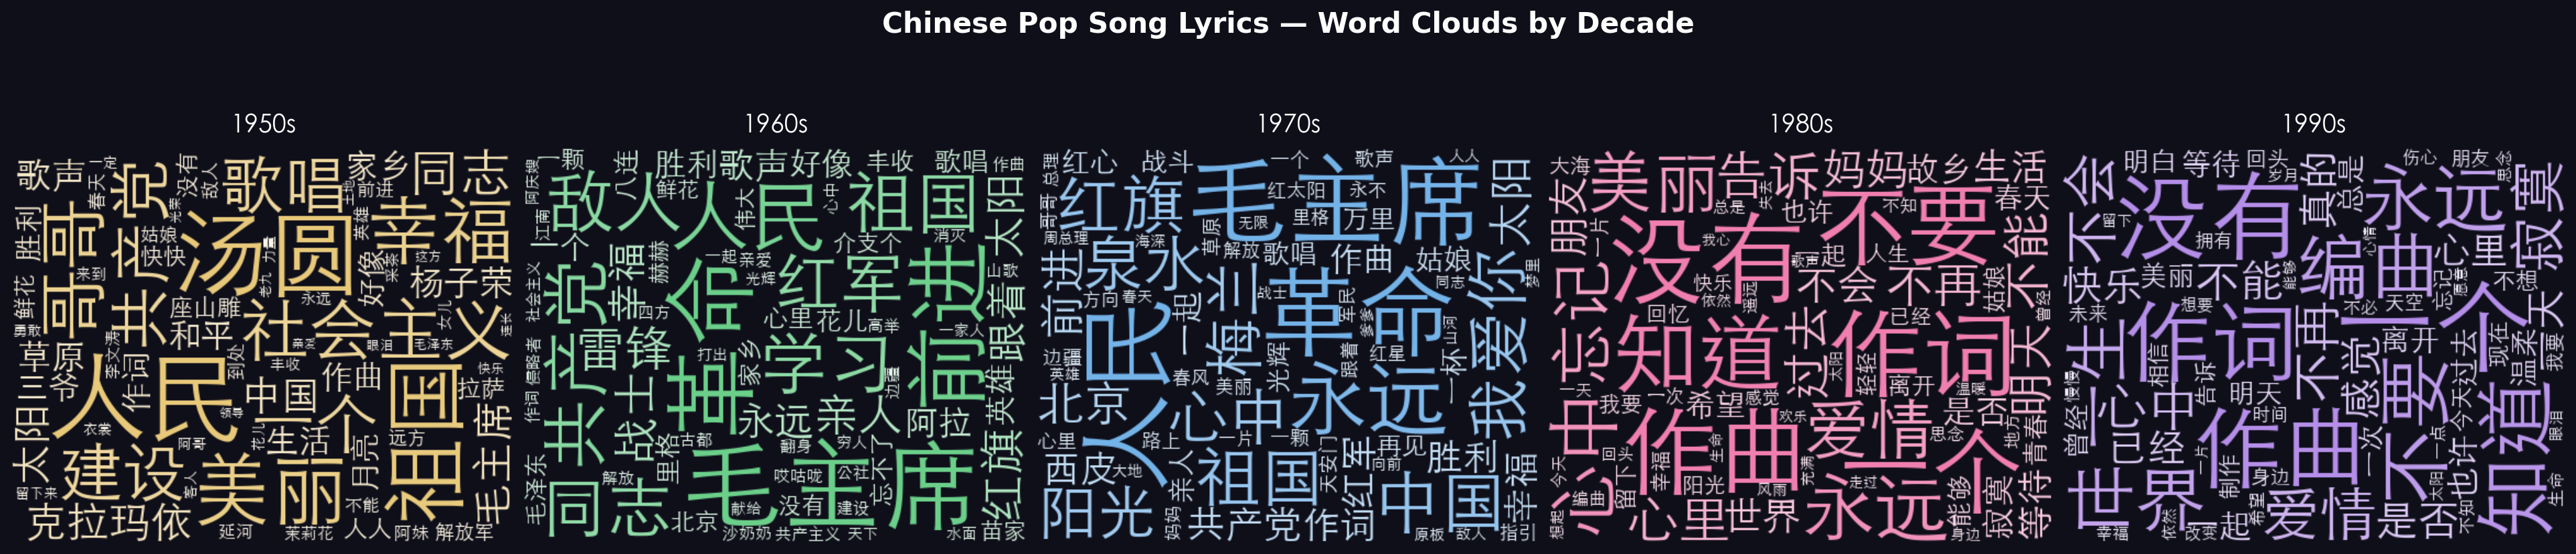
\includegraphics[width=\textwidth, height=0.58\textheight, keepaspectratio]{figures/wordcloud_by_decade.png}
\end{center}

\vspace{0.2em}
\begin{center}
\small
\begin{tabular}{p{2.4cm}p{3.1cm}p{2.75cm}p{2.4cm}p{2.75cm}}
  \textbf{1950s} & \textbf{1960s} & \textbf{1970s} & \textbf{1980s} & \textbf{1990s} \\[4pt]
  the~people\zh{人民}        & Chairman~Mao\zh{毛主席}    & Chairman~Mao\zh{毛主席}  & hometown\zh{故乡}  & myself\zh{自己}   \\[4pt]
  motherland\zh{祖国}        & revolution\zh{革命}        & the~people\zh{人民}      & mama\zh{妈妈}      & world\zh{世界}    \\[4pt]
  bliss\zh{幸福}             & Communist~Party\zh{共产党} & revolution\zh{革命}      & forever\zh{永远}   & solitude\zh{寂寞} \\
\end{tabular}
\end{center}
\end{frame}

%--- Slide 6c: Genre by Decade --------------------------------------------
\begin{frame}{Descriptive Evidence: Genre Composition by Decade}
\begin{columns}[T]
\begin{column}{0.55\textwidth}<1->
  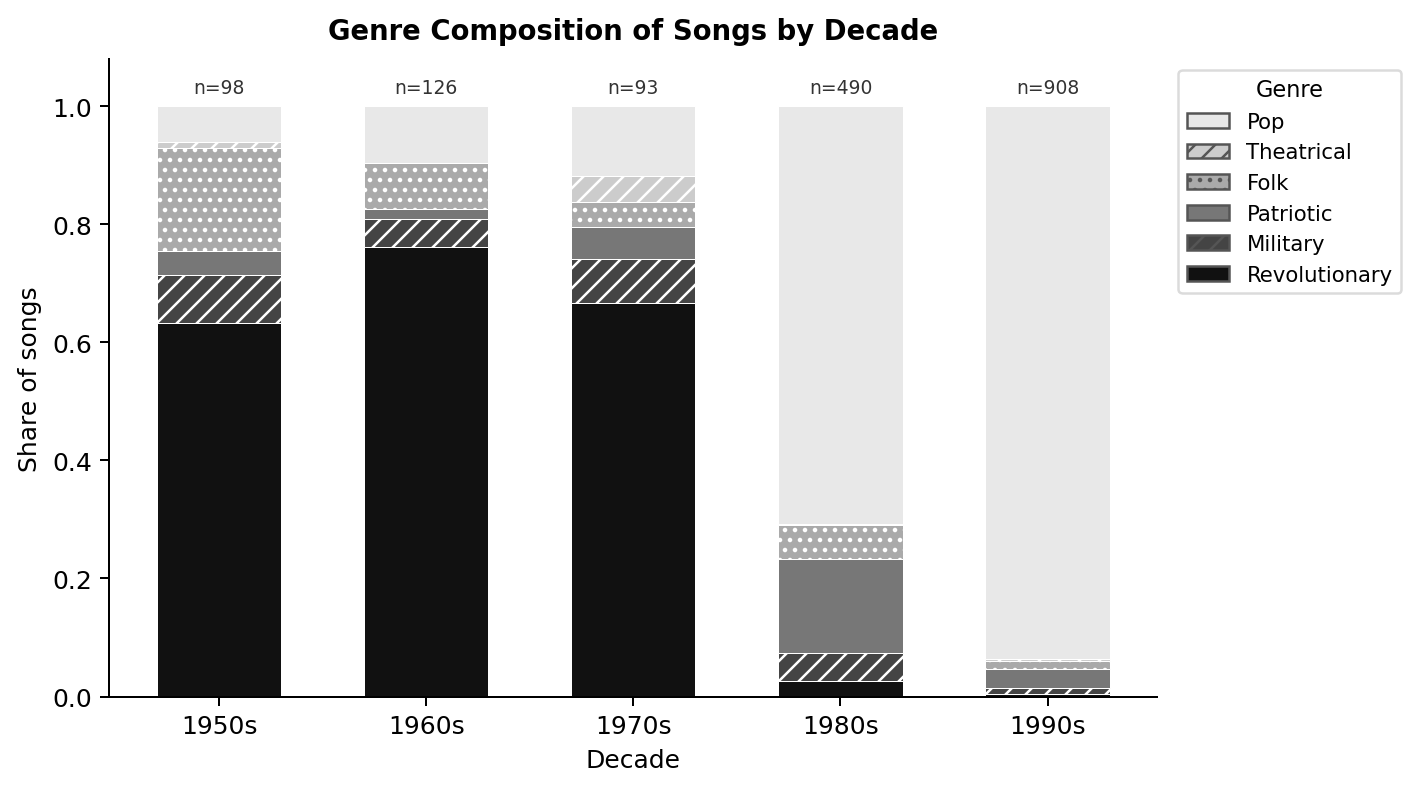
\includegraphics[width=\textwidth, keepaspectratio]{figures/genre/0502/genre_by_decade_v1.png}
\end{column}
\begin{column}{0.43\textwidth}<1->
  \small
  \textbf{Pre-reform dominance:}
  \begin{itemize}
    \item Revolutionary songs account for \textbf{63--76\%} of the sample in the 1950s--70s
  \end{itemize}
  \vspace{0.5em}
  \textbf{Post-reform collapse:}
  \begin{itemize}
    \item By the 1980s, revolutionary share falls to \textbf{3\%}; pop rises to \textbf{71\%} and reaches \textbf{94\%} in the 1990s
  \end{itemize}
\end{column}
\end{columns}
\end{frame}

%--- Slide 6b: Topic Model ------------------------------------------------
\begin{frame}{Descriptive Evidence: Thematic Composition over Time}
  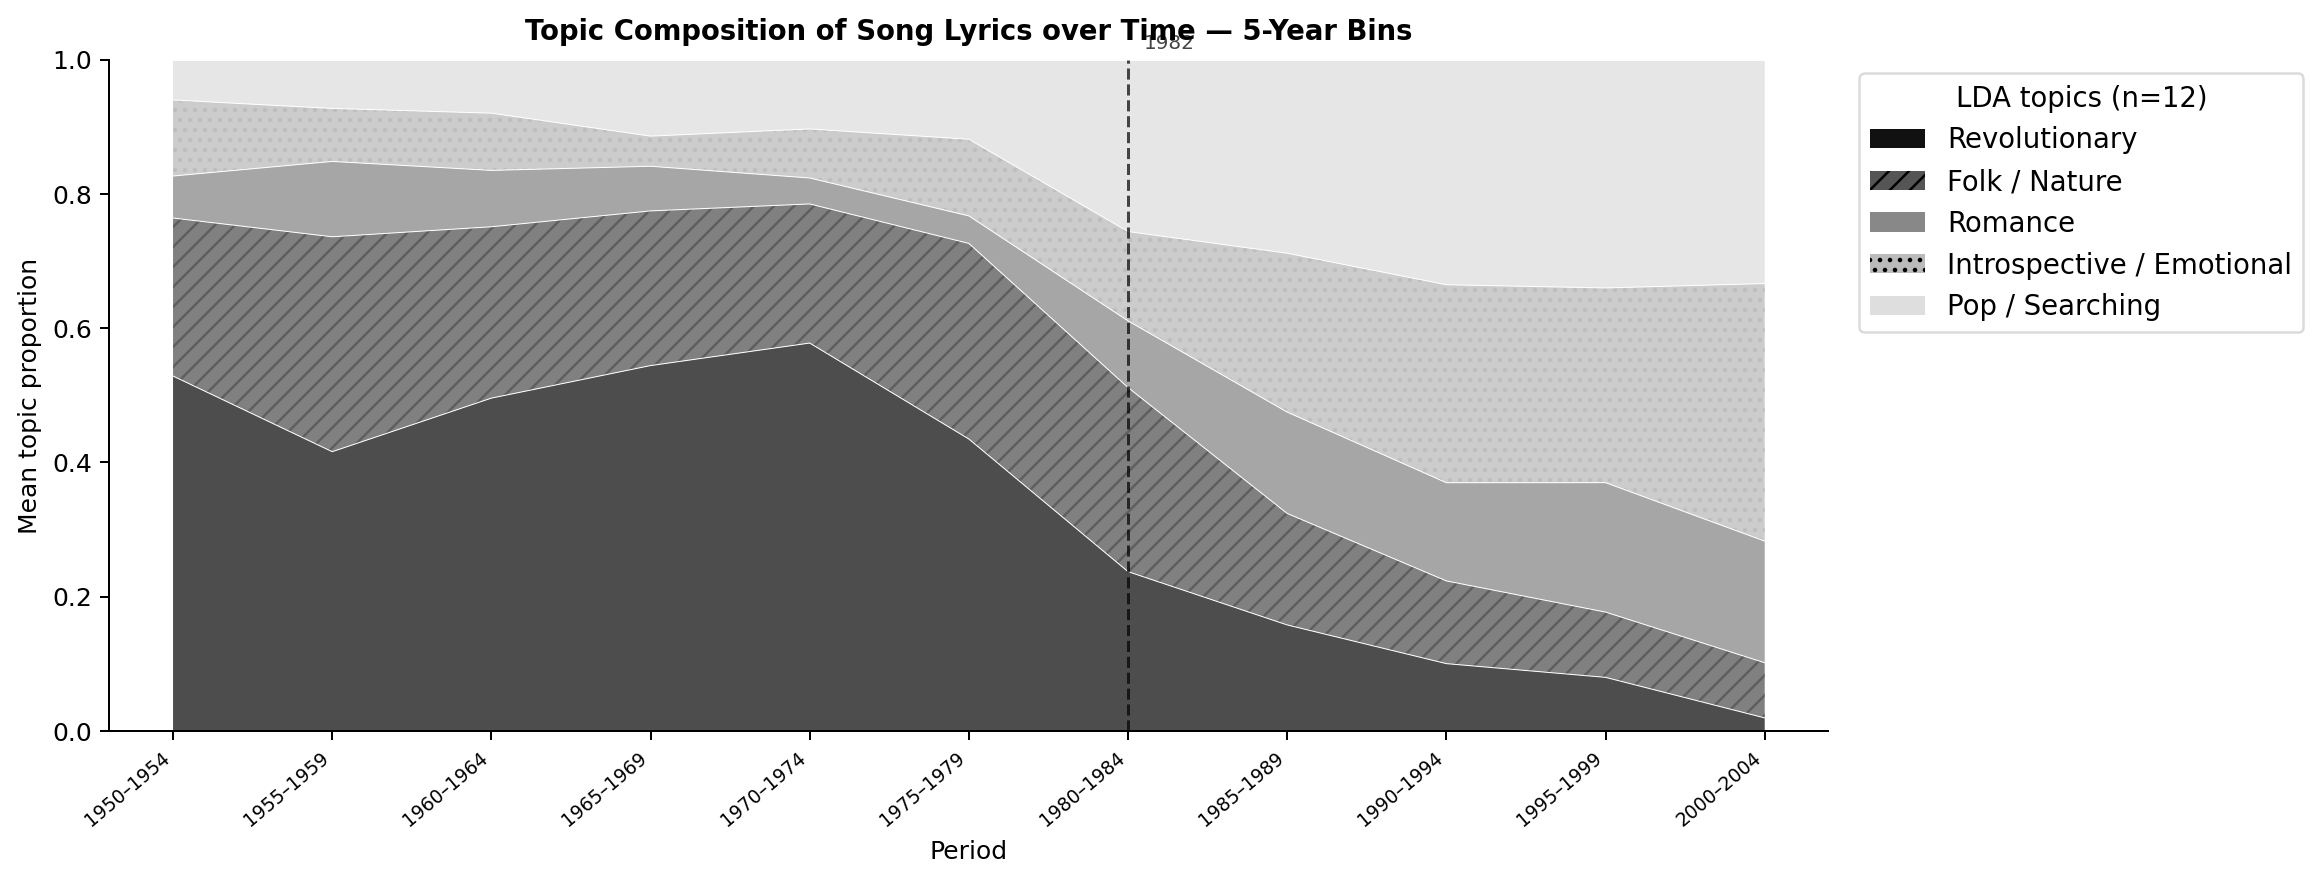
\includegraphics[width=0.83\textwidth, height=0.78\textheight, keepaspectratio]{figures/topic_model/0501/topic_proportions_v1.png}
  
  \small
  \textbf{Compositional shift}
  \begin{itemize}
  \item  Revolutionary content collapses sharply after 1982
  \end{itemize}
  \textbf{Diversification}
  \begin{itemize}
  \item No single theme comes to dominate; the vacated space is filled by multiple genres simultaneously \\[0.4em]
  \end{itemize}
\end{frame}

%--- Slide 6: Measurement Overview -----------------------------------------
\begin{frame}[label=slide-dictmeasures]{Measuring Individualism: Dictionary-based Approaches}

Goal: continuous score per song $\in [-1,+1]$ that consistently captures individualism.

\vspace{0.4em}
  \begin{itemize}
    \item \textbf{Raw Count Net Score}
      $$S_{\text{raw}} = \frac{I - C}{I + C}$$
      Counts of dictionary hits for individualism ($I$) and collectivism ($C$).
    \vspace{0.3em}
    \item \textbf{TF-IDF Net Score}
      $$S_{\text{tfidf}} = \frac{W_I - W_C}{W_I + W_C}$$
      TF-IDF weights over dictionary terms. Down-weights ubiquitous words (e.g., ``we'').
  \end{itemize}
\end{frame}

\begin{frame}{Normalization}
  \textbf{Why this normalisation?}
    \footnotesize
    \begin{enumerate}
      \item \textbf{Controls for song length:} dividing by $I+C$ measures relative balance, not raw counts
      \item \textbf{Bounded in $[-1,+1]$:} pure individualist $= +1$; pure collectivist $= -1$; no dictionary hits $= 0$
      \item \textbf{Symmetric:} same denominator on both sides — no directional inflation
    \end{enumerate}

\vspace{0.4em}
\hyperlink{appendix-indiv-dict}{\beamergotobutton{Individualism Dictionary}}
\hspace{0.3em}
\hyperlink{appendix-collec-dict}{\beamergotobutton{Collectivism Dictionary}}
\end{frame}

\begin{frame}[label=slide-embeddingmeasures]{Measuring Individualism: Embedding Score}

\textbf{Construction:} Word2Vec skip-gram trained on the full lyrics corpus (dim 300, window 5). For each song:
\[
  \text{embedding\_score} = \cos(\bar{v}_{\text{song}},\, \bar{v}_{\text{ind}}) - \cos(\bar{v}_{\text{song}},\, \bar{v}_{\text{col}})
\]
where $\bar{v}_{\text{song}}$ is the mean word vector of the song, and $\bar{v}_{\text{indiv}}$, $\bar{v}_{\text{collec}}$ are centroids of the seed word vectors.

\medskip
\textbf{Why a short seed list?}
\vspace{0.4em}
\hyperlink{appendix-embedding-seeds}{\beamergotobutton{Embedding Seed Words}}
\end{frame}

%--- Slide 7: Descriptive Evidence — Distribution --------------------------
\begin{frame}{Descriptive Evidence: Score Distributions}
\begin{center}
  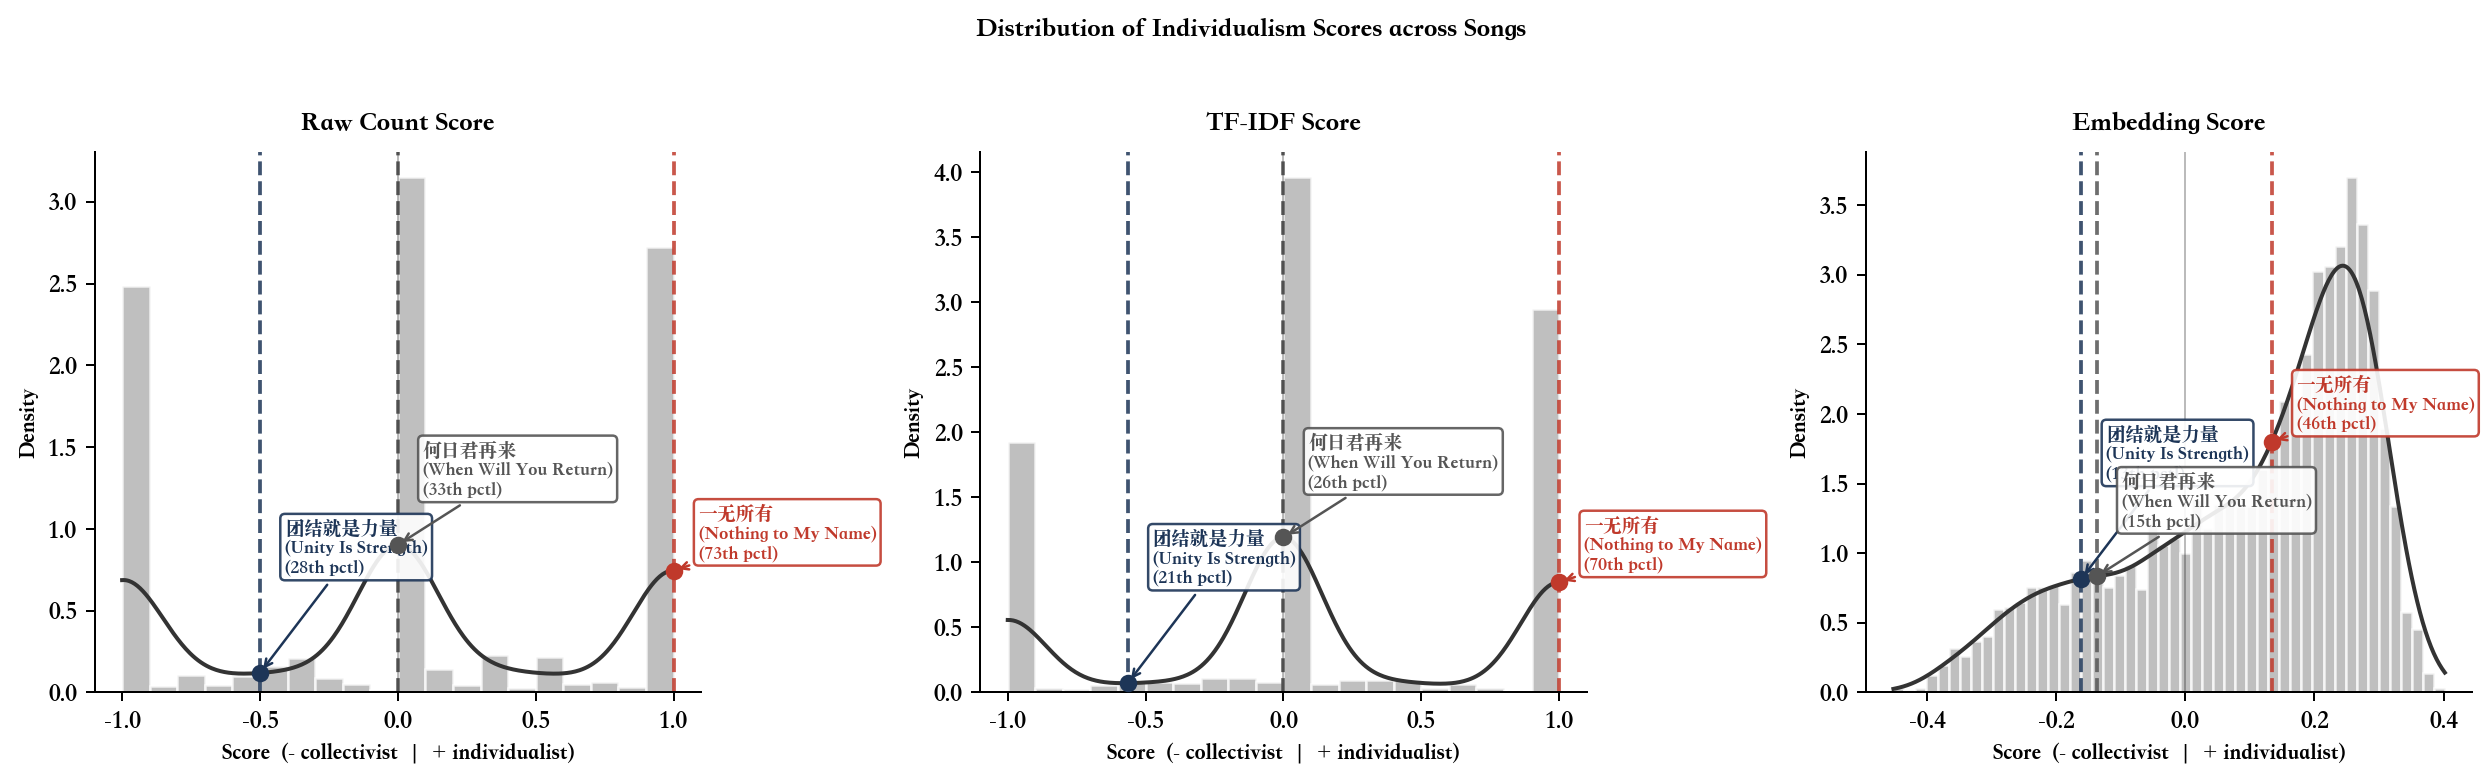
\includegraphics[width=\textwidth, height=\textheight, keepaspectratio]{figures/score_dist/0501/score_distributions_v2.png}
\end{center}

\end{frame}

%--- Slide 8: Descriptive Evidence — Time Trends ---------------------------
\begin{frame}{Descriptive Evidence: Individualism Over Time}

  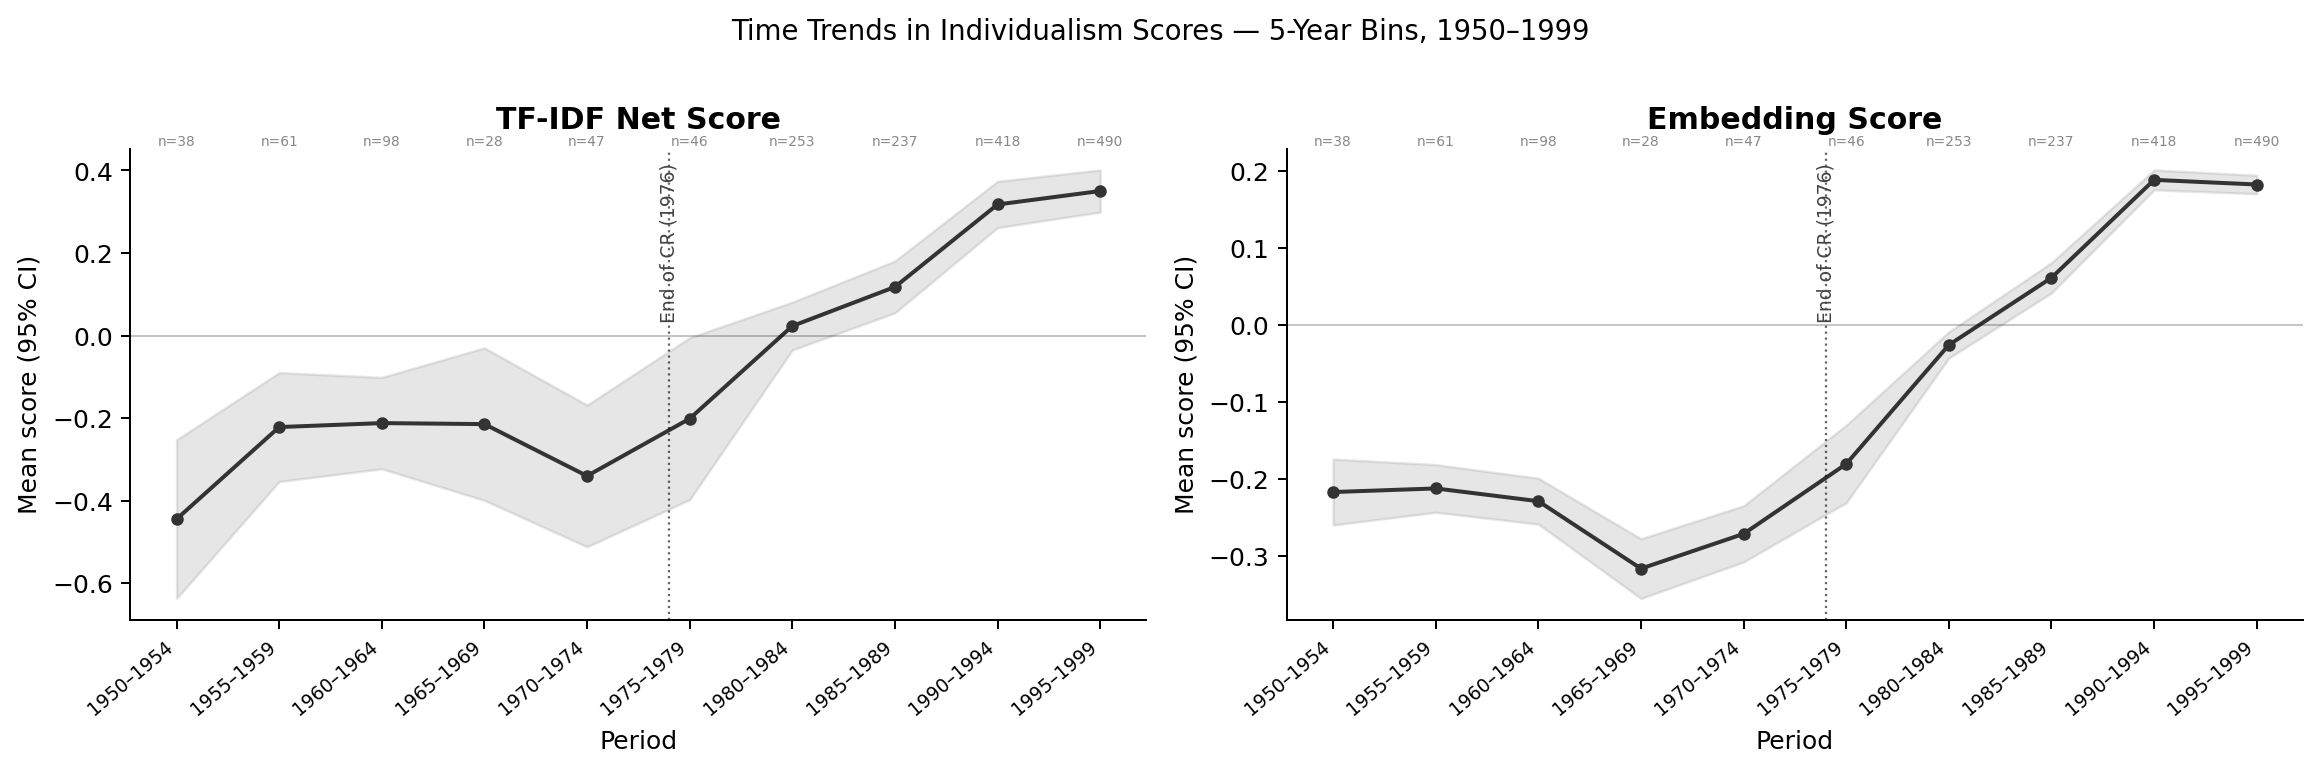
\includegraphics[width=\textwidth, height=\textheight, keepaspectratio]{figures/time_trend/0501/time_trend_v1.png}
\end{frame}

%--- Slide 9: Descriptive Evidence — Space --------------------------------
\begin{frame}{Descriptive Evidence: Individualism Over Space}

  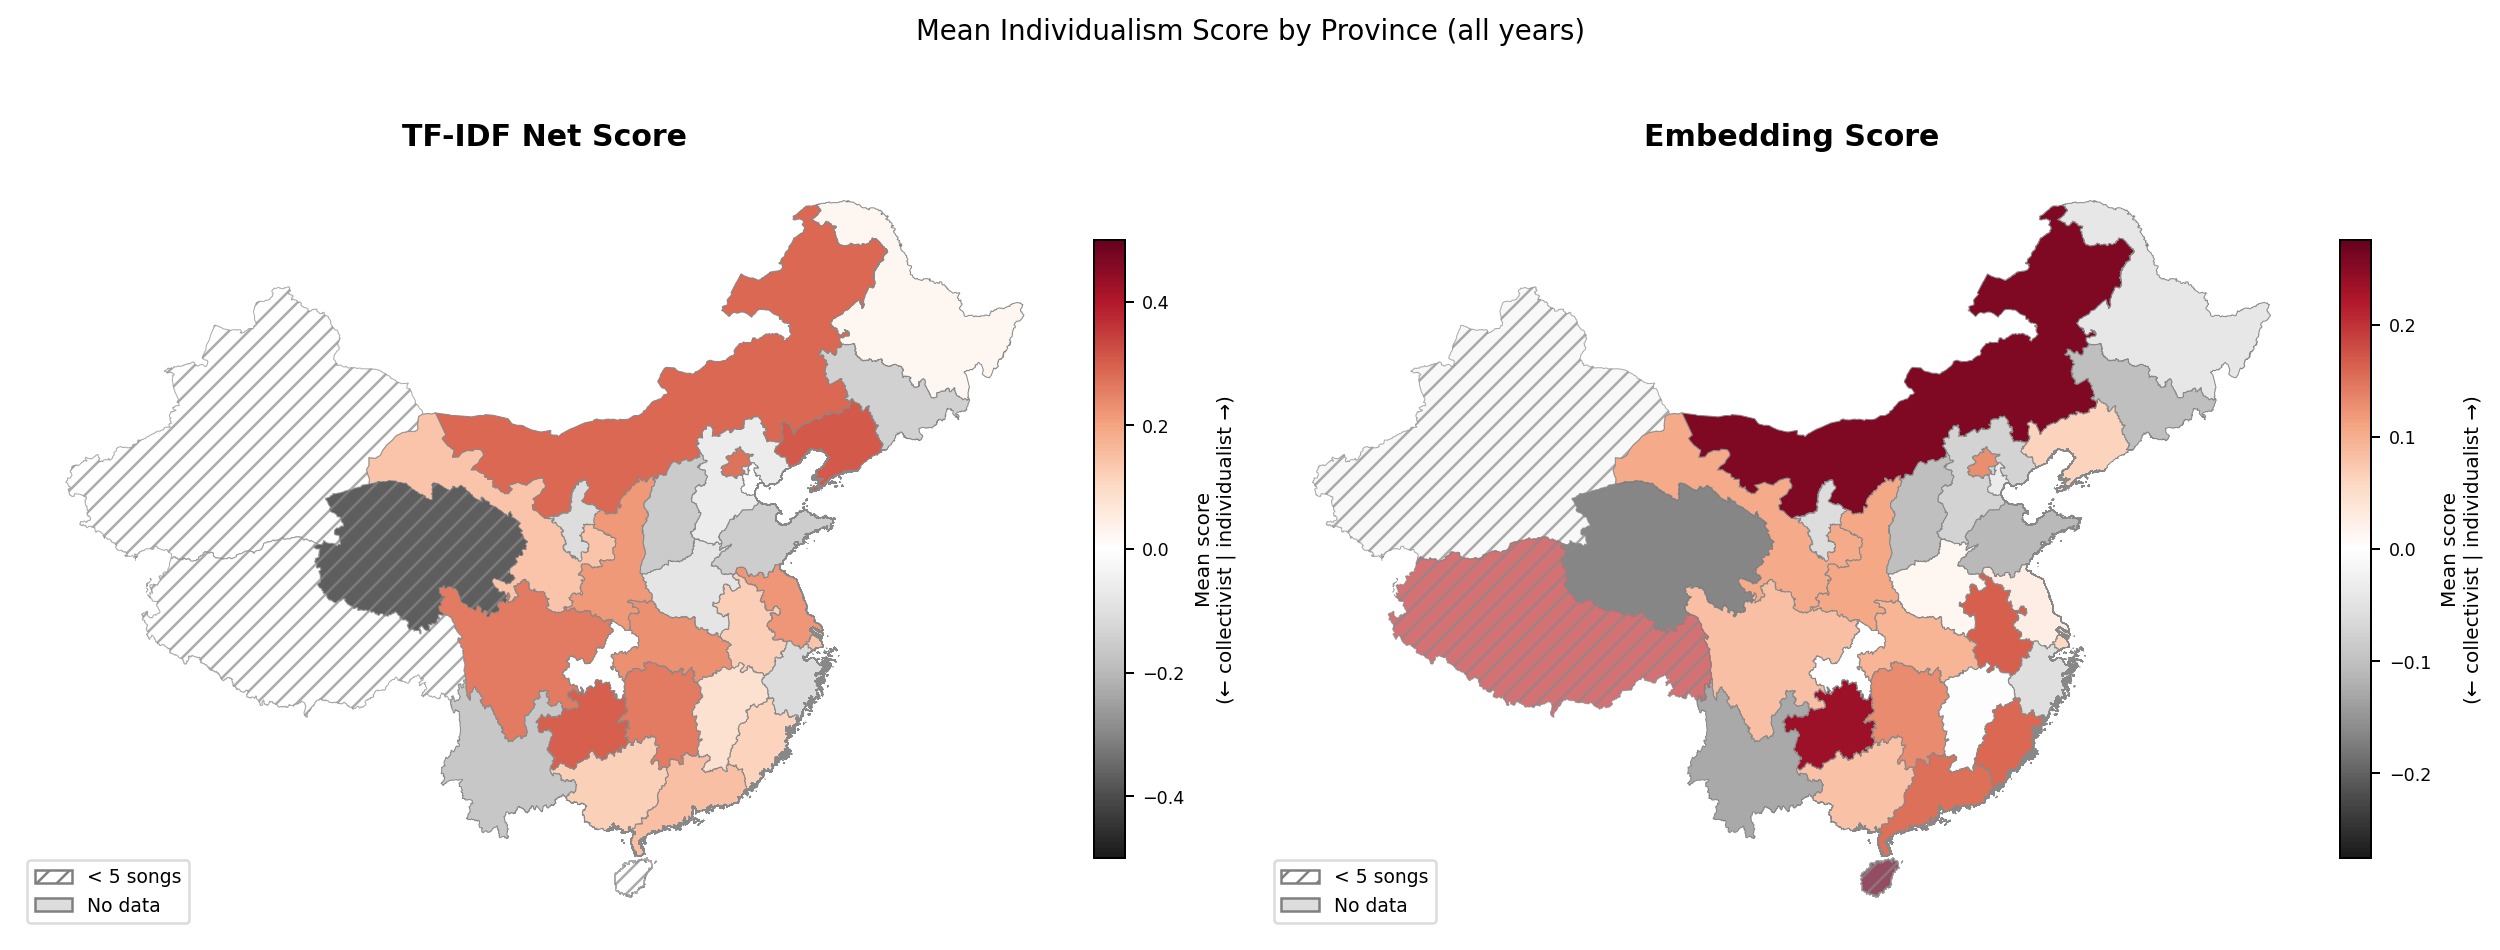
\includegraphics[width=\textwidth, height=\textheight, keepaspectratio]{figures/maps_overall/0501/province_map_v1.png}

\end{frame}

%--- Slide 10: Interpreting the Break -------------------------------------
\begin{frame}{What Could Drive the Break in Trend?}

\begin{itemize}\setlength\itemsep{0.6em}
  \item \textit{Censorship loosening:} content controls relaxed post-1978; previously proscribed personal and romantic themes became permitted.
\bigskip
  \item \textbf{\textit{Economic institutional change}} operates on both sides of the cultural market:
  \begin{itemize}\setlength\itemsep{0.3em}
    \item Supply — decentralization of cultural production gives lyricists new conditions of work and material
    \item Demand — factor-market reform reshapes incentives, hence audience tastes
  \end{itemize}
\end{itemize}

\end{frame}

\begin{frame}{Non-State Firm Share}
\begin{columns}[T]
\begin{column}{0.5\textwidth}<1->
\resizebox{\linewidth}{!}{%
\begin{tabular}{lccc}
\toprule
 & (1) & (2) & (3) \\
 & Raw Count & TF-IDF & Word2Vec \\
\midrule
Share non-state firms  & 0.753  & 0.718  & 0.302\sym{**} \\
                       & (0.465) & (0.352) & (0.063) \\
\midrule
Mean dep.\ var.        & 0.018  & 0.150  & 0.010 \\
Observations           & 1723   & 1723   & 1722 \\
Province FE            & Yes   & Yes   & Yes   \\
Year FE                & Yes   & Yes   & Yes   \\
Area$\times$Year FE    & Yes   & Yes   & Yes   \\
\bottomrule
\end{tabular}%
}
{\tiny Stars: wild-bootstrap $p$-values (Webb, 999~reps). $^{*}p<0.10$, $^{**}p<0.05$, $^{***}p<0.01$.}
\end{column}
\begin{column}{0.45\textwidth}<1->
\begin{itemize}\small
  \item \textbf{Data:} business registration records (\begin{CJK}{UTF8}{gbsn}工商注册信息\end{CJK}) — annual stock of registered firms by ownership type (state, collective, private, individual)
  \item Word2Vec score rises with non-state share; Raw and TF-IDF coefficients are positive but imprecise
\end{itemize}
\end{column}
\end{columns}
\end{frame}

\begin{frame}{Reform Policy}

\textbf{Data — \begin{CJK}{UTF8}{gbsn}北大法宝\end{CJK} (PKU LawInfo)}
\begin{itemize}\small
  \item Comprehensive repository of Chinese legislation and administrative regulations
  \item All provincial/city-level documents, 1970--1990; exclude party, military, and national law categories
\end{itemize}

\vspace{0.35em}
\textbf{Classification pipeline}
\begin{enumerate}\small
  \item Manually define \textbf{25 economic reform categories} {\footnotesize(Chen, Li \& Zhu, 2025)}\\
        {\footnotesize(household responsibility, wage reform, price reform, SOE reform, FDI/SEZ, housing reform, \ldots)}
  \item \textbf{Stage 1 — Gemini 2.5 Flash}: classify each document against the 25 categories; output confidence score (0--100)
  \item \textbf{Stage 2 — Gemini 2.5 Pro}: re-verify borderline cases (confidence 30--75); overrides Stage 1 decision
  \item Aggregate: $\text{ReformCount}_{p,y}$ = cumulative unique reform-related docs in province $p$ through year $y$
\end{enumerate}
{\footnotesize Follows Fang et al.\ (2025) hallucination-robust multi-LLM approach.}

\end{frame}

\begin{frame}{Reform Policy Results}

\large \textbf{Why only 1978--1990?}
\vspace{0.6em}
\normalsize
\begin{itemize}
  \item \textbf{First reform wave}
  \begin{itemize}
    \item  Core institutional break window, later phase potentially confounded with globalization
  \end{itemize}
  \vspace{0.6em}
  \item \textbf{Consistent with main treatment}
  \begin{itemize}
    \item Cadre-replacement instrument captures exposure to the same first wave
  \end{itemize}
  \vspace{0.6em}
  \item Budget constraint
\end{itemize}

\end{frame}

\begin{frame}{Reform Policy Results}

\begin{columns}[T]
\begin{column}{0.5\textwidth}<1->

\resizebox{\linewidth}{!}{%
\begin{tabular}{lccc}
\toprule
 & (1) & (2) & (3) \\
 & Raw Count & TF-IDF & Word2Vec \\
\midrule
\multicolumn{4}{l}{\textit{Panel A: $\ln$Distance$\times$Post only}} \\[2pt]
ReformCount  & 0.0005\sym{**}  & 0.0003\sym{**}  & 0.0002\sym{*}   \\
             & (0.0001)        & (0.0001)        & (0.0000)        \\
\addlinespace[5pt]
\multicolumn{4}{l}{\textit{Panel B: Full controls (GDP, CultRev, Trade, Distance)}} \\[2pt]
ReformCount  & 0.0005\sym{*}   & 0.0003\sym{*}   & 0.0002\sym{*}   \\
             & (0.0001)        & (0.0001)        & (0.0000)        \\
\midrule
Mean dep.\ var.      & $-$0.226  & $-$0.051  & $-$0.092  \\
Observations         & 845       & 845       & 844       \\
Province FE          & \multicolumn{3}{c}{Yes} \\
Year FE              & \multicolumn{3}{c}{Yes} \\
Area$\times$Year FE  & \multicolumn{3}{c}{Yes} \\
\bottomrule
\end{tabular}%
}

{\tiny Stars: wild-bootstrap $p$-values (Webb, 999~reps). $^{*}p<0.10$, $^{**}p<0.05$, $^{***}p<0.01$.}

\end{column}
\begin{column}{0.45\textwidth}<1->

\vspace{0.3em}
\begin{itemize}\small
  \item Pre-1978 province-years assigned $\text{ReformCount}=0$
  \item Post-1990 observations dropped
  \vspace{0.4em}
  \item Lower mean dep.\ var.\ relative to main results consistent with the upward individualism trend in the data
\end{itemize}

\end{column}
\end{columns}

\end{frame}

%--- Slide 11: Identification Strategy ------------------------------------
\begin{frame}{Empirical Strategy: Deng's 1982--1984 Cadre Replacement}

\textbf{Core idea:} exploit \textbf{differential adoption} of market reforms across provinces via the 1982–84 cadre replacement campaign.
\begin{itemize}
    \item Deng Xiaoping's 1982--1984 administrative reforms systematically replaced Maoist-era cadres (\textit{``three types of persons''}) with younger, reform-oriented technocrats
\end{itemize}
\vspace{0.4em}
  \textbf{Data sources}
  \begin{itemize}\small
    \item \textit{China's Organizational History Dataset} — official career profiles of provincial-level officials
    \item \textit{China Political Elite Dataset} (Kou \& Zang) — biographical records used to classify Maoist-era affiliations
    \item Pre-reform (1981) vs.\ post-reform (1984) snapshots identify turnover intensity per province
  \end{itemize}

\end{frame}

%--- Slide 20b: Provincial Leader Data ------------------------------------
\begin{frame}{Identification: Reform Exposure Measure}
\textbf{Treatment — \texttt{ReformExposure}$_{p,y}$:}
\begin{itemize}
 \item $\text{Intensity}_p = 100\times\dfrac{\#\text{Maoist}_{p,1981} - \#\text{Maoist}_{p,1984}}{\#\text{Maoist}_{p,1981}}$
    \item Province-level percentage drop in Maoist cadres, 1981--1984
  \item $\uparrow$ \texttt{ReformExposure}$_{p,y}$ $\Rightarrow$ $\uparrow$ displacement of Mao-era leadership $\Rightarrow$ \alert{$\uparrow$ reform exposure}
  \item Interacted with a post-1982 indicator
\end{itemize}

\vspace{0.4em}
\textbf{Key identifying assumption:}
cadre replacement should not be correlated with local cultural development
\begin{itemize}
  \item Top-down, not driven by local conditions
  \item Institutional response to political screening constraints
\end{itemize}

\end{frame}

%--- Slide 10: Specification -----------------------------------------------
\begin{frame}{Empirical Strategy: Specification}

\textbf{Baseline regression:}
\begin{equation*}
  Y_{s(p,y)} = \beta\,(\text{Intensity}_p \times \text{Post}_y)
  + \mathbf{X}_p'\boldsymbol{\gamma}\,\text{Post}_y
  + \lambda_p + \sigma_y + \delta_{r(p),y} + \varepsilon_{s(p,y)}
\end{equation*}
\vspace{-0.3em}
where $s(p,y)$ indexes song $s$ by a lyricist born in province $p$, released in year $y$; $r(p)$ denotes the macro-region of province $p$.

\vspace{0.8em}
\textbf{Control variables} $\mathbf{X}_p$ (all 1981 pre-reform baselines, interacted with $\text{Post}_y$):
\begin{itemize}\small
  \item $\ln\text{GDP}_{1981,p}$ — pre-reform income level
  \item $\text{CultRevDeaths}_p$ — Cultural Revolution deaths as a share of population
  \item $\ln\text{ImExports}_{1981,p}$ — pre-reform trade openness
  \item $\ln\text{Distance}_p \times \text{Post}_y$ — distance to Beijing
\end{itemize}
\end{frame}



%--- Slide 11: Results ----------------------------------------------------
\begin{frame}[shrink=5]{Results}
\begin{columns}[T]

%-- Left: table -----------------------------------------------------------
\begin{column}{0.5\textwidth}<1->
\resizebox{\linewidth}{!}{%
\begin{tabular}{lccc}
\toprule
 & (1) & (2) & (3) \\
 & Raw Count & TF-IDF & Word2Vec \\
\midrule
\multicolumn{4}{l}{\textit{Panel A: Baseline}} \\[2pt]
ReformExposure  & 0.016          & 0.042\sym{**}  & 0.013\sym{*}   \\
                & (0.021)        & (0.016)        & (0.006)        \\
\addlinespace[6pt]
\multicolumn{4}{l}{\textit{Panel B: + Lyricist FE}} \\[2pt]
ReformExposure  & 0.005          & 0.018          & 0.003          \\
                & (0.069)        & (0.065)        & (0.016)        \\
\midrule
Mean dep.\ var.     & 0.018 & 0.150 & 0.010 \\
Observations        & 1722  & 1722  & 1721  \\
Province FE         & Yes   & Yes   & Yes   \\
Year FE             & Yes   & Yes   & Yes   \\
Area$\times$Year FE & Yes   & Yes   & Yes   \\
\bottomrule
\end{tabular}%
}
{\tiny Stars: wild-bootstrap $p$-values (Webb, 999~reps). $^{*}p<0.10$, $^{**}p<0.05$, $^{***}p<0.01$.}
\end{column}

%-- Right: remarks --------------------------------------------------------
\begin{column}{0.45\textwidth}<1->

\smallskip
\begin{itemize}
  \item TF-IDF significant at 5\%
  \item Word2Vec significant at 10\%

\medskip
\item Results disappear once lyricist fixed effects are added

$\Rightarrow$ reform effect likely driven by change in composition from the supply side
\end{itemize}
\end{column}

\end{columns}
\end{frame}

%--- Slide 24: Event Study ------------------------------------------------
\begin{frame}{Event Study}
\begin{center}
  \includegraphics[width=\textwidth, height=0.82\textheight, keepaspectratio]{../../figures/event_study/0501/event_study_specC_v6.png}
\end{center}
\end{frame}

%--- Slide 13: Discussion --------------------------------------------------
\begin{frame}{Discussion \& Interpretation}

  \textbf{Summary of findings:}
  \begin{itemize}
    \item Robust positive relationship between reform intensity and lyrical individualism across three of four measures
  \item Negative coeff. on GDP interaction \\
  $\Rightarrow$ Provinces that were better-off during the CR were \emph{also} those with higher collectivism, and experienced a \emph{smaller} individualism rise under reform. Suggests reform operated through structural change rather than income growth alone.
  \end{itemize}
\end{frame}

%--- Slide 14: Next Steps --------------------------------------------------
\begin{frame}{Next Steps and Limitations}
\begin{columns}[T]
\begin{column}{0.50\textwidth}<1->
  \textbf{Next steps}
  \begin{itemize}\small
    \item \textbf{Decompose the net score:} run individualism and collectivism regressions separately to identify whether the rise is driven by more individualist content, less collectivist content, or both
    \item \textbf{Reform exposure duration:} exploit variation in how many years a lyricist was exposed to the reform environment before writing
  \end{itemize}
\end{column}
\begin{column}{0.46\textwidth}<1->
  \textbf{Limitations}
  \begin{itemize}\small
    \item \textbf{Supply vs.\ demand:} cannot distinguish whether individualist content rose because new lyricists brought different values (supply) or because audiences demanded it — lyricist FE results are suggestive but not conclusive
    \item \textbf{Censorship floor:} overtly individualist content may have been suppressed even post-1978, so the measured effect is likely a lower bound on true cultural change
  \end{itemize}
\end{column}
\end{columns}
\end{frame}

%--- Slide 15: Conclusion --------------------------------------------------
\begin{frame}{Conclusion}

\textbf{What we do}
\begin{itemize}
  \item First large-scale text-as-data measure of individualism in Chinese popular culture, 1950--2000
\end{itemize}

\vspace{0.5em}
\textbf{What we find}
\begin{itemize}
  \item Sharp rise in lyrical individualism coinciding with the post-1978 reform era
  \item Provinces more exposed to Deng's 1982--84 cadre replacement show significantly greater individualism in song lyrics
  \item Reform policy count independently confirms the pattern across all three measures
\end{itemize}

\vspace{0.5em}
\textbf{What it means}
\begin{itemize}
  \item Economic institution reform reshapes cultural values \textit{even in a censored environment}
  \item Markets cultivate individualism through compositional change in cultural production
\end{itemize}

\end{frame}

%--- Appendix ---------------------------------------------------------------
\appendix

% Reset overlays so appendix items render fully visible
\beamerdefaultoverlayspecification{}

%-- Individualism Dictionary: Chinese --
\begin{frame}[label=appendix-indiv-dict]{Appendix: Individualism Dictionary}
\footnotesize
\begin{columns}[T]
\begin{column}{0.50\textwidth}<1->
  \textbf{Self (2)} \\
  \begin{CJK}{UTF8}{gbsn}自己、自我\end{CJK}

  \smallskip
  \textbf{Agency / Choice (7)} \\
  \begin{CJK}{UTF8}{gbsn}我想、我想要、我只想、我要、我选择、我不想、我不愿\end{CJK}

  \smallskip
  \textbf{Defiance / Attitude (7)} \\
  \begin{CJK}{UTF8}{gbsn}不在乎、无所谓、不后悔、不低头、随性、随我、随心\end{CJK}

  \smallskip
  \textbf{Freedom (2)} \\
  \begin{CJK}{UTF8}{gbsn}自由、无拘无束\end{CJK}
\end{column}
\begin{column}{0.48\textwidth}<1->
  \textbf{Solitude / Inner Life (6)} \\
  \begin{CJK}{UTF8}{gbsn}独自、独立、一个人、孤独、孤单、寂寞\end{CJK}

  \smallskip
  \textbf{Wandering (3)} \\
  \begin{CJK}{UTF8}{gbsn}远方、流浪、漂泊\end{CJK}

  \smallskip
  \textit{27 terms total.}
\end{column}
\end{columns}

\vspace{0.4em}
\hyperlink{slide-dictmeasures}{\beamerreturnbutton{Back}}
\hfill
\hyperlink{appendix-indiv-dict-en}{\beamergotobutton{English Translations}}
\hspace{0.3em}
\hyperlink{appendix-collec-dict}{\beamergotobutton{Collectivism Dictionary}}
\end{frame}

%-- Individualism Dictionary: English --
\begin{frame}[label=appendix-indiv-dict-en]{Appendix: Individualism Dictionary (English)}
\footnotesize
\begin{columns}[T]
\begin{column}{0.50\textwidth}<1->
  \textbf{Self} \\
  \textit{oneself, self}

  \smallskip
  \textbf{Agency / Choice} \\
  \textit{I want, I want to, I only want, I will, I choose, I don't want, I'm unwilling}

  \smallskip
  \textbf{Defiance / Attitude} \\
  \textit{don't care, doesn't matter, no regrets, won't bow down, follow my nature, as I please, follow my heart}

  \smallskip
  \textbf{Freedom} \\
  \textit{freedom, unrestrained}
\end{column}
\begin{column}{0.48\textwidth}<1->
  \textbf{Solitude / Inner Life} \\
  \textit{alone, independent, by myself, solitude, loneliness (lonely), loneliness}

  \smallskip
  \textbf{Wandering} \\
  \textit{faraway, roaming, drifting}
\end{column}
\end{columns}

\vspace{0.4em}
\hyperlink{appendix-indiv-dict}{\beamerreturnbutton{Chinese Terms}}
\hfill
\hyperlink{appendix-collec-dict}{\beamergotobutton{Collectivism Dictionary}}
\end{frame}

%-- Collectivism Dictionary: Chinese --
\begin{frame}[label=appendix-collec-dict]{Appendix: Collectivism Dictionary}
\footnotesize
  \textbf{Group Pronouns (6)} \\
  \begin{CJK}{UTF8}{gbsn}我们、咱、咱们、大家、众人、全民\end{CJK}

  \smallskip
  \textbf{Joint Action / Solidarity (9)} \\
  \begin{CJK}{UTF8}{gbsn}一起、一同、共同、同在、同心、齐心、同行、团结、一条心\end{CJK}

  \smallskip
  \textbf{Collective Entities (7)} \\
  \begin{CJK}{UTF8}{gbsn}集体、群体、团体、团队、队伍、社里、人民\end{CJK}

  \smallskip
  \textit{22 terms total.}

\vspace{0.4em}
\hyperlink{appendix-indiv-dict}{\beamergotobutton{Individualism Dictionary}}
\hfill
\hyperlink{appendix-collec-dict-en}{\beamergotobutton{English Translations}}
\hspace{0.3em}
\hyperlink{slide-dictmeasures}{\beamerreturnbutton{Back}}
\end{frame}

%-- Collectivism Dictionary: English --
\begin{frame}[label=appendix-collec-dict-en]{Appendix: Collectivism Dictionary (English)}
\footnotesize
  \textbf{Group Pronouns} \\
  \textit{we, we (informal), we (inclusive), everyone, all people, all citizens}

  \smallskip
  \textbf{Joint Action / Solidarity} \\
  \textit{together, jointly, in common, together in presence, united in heart, of one mind, travel together, unity, of one mind}

  \smallskip
  \textbf{Collective Entities} \\
  \textit{collective, group, organization, team, troop, commune, the people}

  \smallskip
  \textit{22 terms total.}

\vspace{0.4em}
\hyperlink{appendix-collec-dict}{\beamerreturnbutton{Chinese Terms}}
\hfill
\hyperlink{appendix-indiv-dict}{\beamergotobutton{Individualism Dictionary}}
\end{frame}

%-- Embedding Seeds: Chinese --
\begin{frame}[label=appendix-embedding-seeds]{Appendix: Embedding Seed Words}
\footnotesize
  \textbf{Individualism seeds (7)} \\
  \begin{CJK}{UTF8}{gbsn}自己、自由、孤独、寂寞、漂泊、流浪、一个人\end{CJK}

  \medskip
  \textbf{Collectivism seeds (5)} \\
  \begin{CJK}{UTF8}{gbsn}咱、大家、团结、共同、一起\end{CJK}

\vspace{0.4em}
\hyperlink{slide-embeddingmeasures}{\beamerreturnbutton{Back}}
\hfill
\hyperlink{appendix-embedding-seeds-en}{\beamergotobutton{English Translations}}
\end{frame}

%-- Embedding Seeds: English --
\begin{frame}[label=appendix-embedding-seeds-en]{Appendix: Embedding Seed Words (English)}
\footnotesize
  \textbf{Individualism seeds (7)} \\
  \textit{oneself, freedom, solitude, loneliness, drifting, roaming, alone}

  \medskip
  \textbf{Collectivism seeds (5)} \\
  \textit{we (informal), everyone, unity, in common, together}

\vspace{0.4em}
\hyperlink{appendix-embedding-seeds}{\beamerreturnbutton{Chinese Terms}}
\hfill
\hyperlink{slide-embeddingmeasures}{\beamergotobutton{Embedding Score Slide}}
\end{frame}

%--- References ---------------------------------------------------------------
\begin{frame}[allowframebreaks]{References}
\tiny
\setlength{\parskip}{4pt}

\textbf{Alesina, A. and N. Fuchs-Sch\"{u}ndeln} (2007). ``Good-Bye Lenin (or Not?): The Effect of Communism on People's Preferences.'' \textit{American Economic Review}, 97(4), 1507--1528.

\textbf{Bazzi, S., M. Fiszbein, and M. Gebresilasse} (2020). ``Frontier Culture: The Roots and Persistence of `Rugged Individualism' in the United States.'' \textit{Econometrica}, 88(6), 2329--2368.

\textbf{Bernstein, T.P.} (1977). \textit{Up to the Mountains and Down to the Villages: The Transfer of Youth from Urban to Rural China}. Yale University Press.

\textbf{Chen, H., B. Li, and X. Zhu} (2025). ``Bottom-Up Institutional Change and Growth in China.'' SSRN Working Paper 5097745.

\textbf{Fang, H., M. Li, and G. Lu} (2025). ``Decoding China's Industrial Policies.'' NBER Working Paper No.\ 33814.

\textbf{Giuliano, P. and A. Spilimbergo} (2014). ``Growing Up in a Recession.'' \textit{Review of Economic Studies}, 81(2), 787--817.

\textbf{Gorodnichenko, Y. and G. Roland} (2017). ``Culture, Institutions, and the Wealth of Nations.'' \textit{Review of Economics and Statistics}, 99(3), 402--416.

\textbf{Gorin, C., S. Heblich, and Y. Zylberberg} (2025). ``State of the Art: Economic Development Through the Lens of Paintings.'' NBER Working Paper No.\ 33976.

\textbf{Kou, C. and X. Zang}. \textit{China Political Elite Dataset}.

\textbf{Lin, J.Y.} (1992). ``Rural Reforms and Agricultural Growth in China.'' \textit{American Economic Review}, 82(1), 34--51.

\textbf{Michel, J.-B. et al.} (2011). ``Quantitative Analysis of Culture Using Millions of Digitized Books.'' \textit{Science}, 331(6014), 176--182.

\textbf{Michalopoulos, S. and C. Rauh} (2024). ``Movies.'' NBER Working Paper No.\ 32220.

\textbf{Naughton, B.} (2007). \textit{The Chinese Economy: Transitions and Growth}. MIT Press.

\textbf{Talhelm, T., X. Zhang, S. Oishi, C. Shimin, D. Duan, X. Lan, and S. Kitayama} (2014). ``Large-Scale Psychological Differences Within China Explained by Rice Versus Wheat Agriculture.'' \textit{Science}, 344(6184), 603--608.

\textbf{Voth, H.-J. and D. Yanagizawa-Drott} (2024). ``Images.'' Working paper, University of Zurich.

\textbf{Weigand, M., C. Mohr, and D. Cantoni} (2025). ``Identity and Institutional Change: Evidence from First Names in Germany, 1700--1850.'' CESifo Working Paper No.\ 12155.

\end{frame}

\end{document}
